\documentclass[11pt,a4paper]{article}

\usepackage[utf8]{inputenc}
\usepackage[T1]{fontenc}
\usepackage{lmodern}
\usepackage[margin=2.3cm]{geometry}
\usepackage{amsmath,amssymb}
\usepackage{graphicx}
\usepackage{booktabs}
\usepackage{tabularx}
\usepackage{xcolor}
\usepackage{enumitem}
\usepackage{float}
\usepackage{caption}
\usepackage{listings}
\usepackage{tikz}
\usetikzlibrary{arrows.meta,positioning,fit,backgrounds}
\usepackage[colorlinks=true,linkcolor=nsblue,urlcolor=nsblue,citecolor=nsblue]{hyperref}

\definecolor{nsblue}{HTML}{4355DB}
\definecolor{nsteal}{HTML}{168C79}
\definecolor{nsamber}{HTML}{C88728}
\definecolor{nsink}{HTML}{171923}
\definecolor{nsmuted}{HTML}{7B8190}
\definecolor{nsline}{HTML}{E9EBF0}
\definecolor{nscanvas}{HTML}{F7F8FA}

\lstset{
  basicstyle=\ttfamily\small, columns=fullflexible, breaklines=true,
  backgroundcolor=\color{nscanvas}, frame=single, rulecolor=\color{nsline},
  keywordstyle=\color{nsblue}\bfseries, commentstyle=\color{nsmuted}, stringstyle=\color{nsteal},
  xleftmargin=4pt, xrightmargin=4pt, aboveskip=8pt, belowskip=8pt
}

\setlist{itemsep=2pt, topsep=4pt}
\captionsetup{font=small, labelfont=bf}
\graphicspath{{figures/}}

\newcommand{\code}[1]{\texttt{#1}}

\title{\textbf{Northstar: an Autonomous Data Analyst Agent}\\[4pt]
\large Machine Learning course project -- technical report and demonstration guide}
\author{YOUR NAME\\ \small Course: COURSE NAME \quad Supervisor: PROFESSOR NAME}
\date{November 2026}

\begin{document}
\maketitle

\begin{abstract}
\noindent
Business users often hold valuable tabular data (sales exports, spreadsheets) but lack the time or skills to
profile it, check its quality, detect unusual events and summarise what changed. This project builds an
\emph{autonomous data analyst}: the user uploads a CSV or Excel file and the system automatically infers the
structure of the table, scores its data quality, cleans it, aggregates transactions into time series, detects
anomalies with statistical and machine-learning models, produces a short-term forecast, and presents the results
in a web dashboard where questions can be asked in plain English. The MVP is evaluated on the public
Superstore sales dataset (9{,}994 orders) and on a labelled anomaly benchmark (NYC taxi demand). On the
benchmark, the selected detector (MSTL decomposition with a robust z-score) reaches an F1 score of $0.429$ versus
$0.201$ for the seasonal-difference baseline; on Superstore with injected anomalous orders, an Isolation Forest with
a profit-margin feature recovers $100\%$ of the injected rows while flagging only $1\%$ of the table.
\end{abstract}

\tableofcontents
\newpage

%-----------------------------------------------------------------------------
\section{Problem statement and objectives}

A typical analyst workflow on a new dataset is repetitive: load the file, understand which columns are dates,
amounts or categories, look for missing values and duplicates, compute totals and trends, look for anything
unusual, and write a summary. The goal of this project is to automate that workflow end to end.

\paragraph{MVP scope.} The minimum viable product must:
\begin{enumerate}
  \item accept a CSV or Excel upload;
  \item profile the dataset (column types, statistics, missing values, duplicates) and score its quality;
  \item answer natural-language questions with numbers taken from the data;
  \item show statistics and interactive visualisations;
  \item detect anomalies with machine learning;
  \item generate a written summary of findings.
\end{enumerate}
Forecasting is included as a first version; scheduling, alerts, SQL sources and a large-language-model (LLM)
reasoning layer are planned extensions (Section~\ref{sec:future}).

\paragraph{Design principles.}
\begin{itemize}
  \item \textbf{Evidence first}: every answer shown to the user is computed from the table and comes with the
        numbers that support it.
  \item \textbf{Graceful degradation}: a failing model becomes a warning in the report instead of crashing the
        application.
  \item \textbf{Separation of concerns}: the dashboard never contains ML logic; it calls the analysis package.
\end{itemize}

%-----------------------------------------------------------------------------
\section{Data}

\subsection{Superstore sales (main dataset)}
The main dataset is the public \emph{Superstore} retail dataset
(\href{https://huggingface.co/datasets/An-j96/SuperstoreData}{Hugging Face: An-j96/SuperstoreData}).
It contains \textbf{9{,}994 order lines} and \textbf{21 columns} covering orders placed between
\textbf{3 January 2014 and 30 December 2017}: order and ship dates, customer and product identifiers,
segment, region, category and sub-category, and the four numeric measures \code{Sales}, \code{Quantity},
\code{Discount} and \code{Profit}. Total sales are \$2{,}296{,}919 and total profit \$286{,}409
(a 12.5\% margin).

\subsection{NYC taxi demand (anomaly benchmark)}
Superstore has no ground-truth anomaly labels, so detectors are also evaluated on the NYC taxi passenger series
from the Numenta Anomaly Benchmark (NAB): half-hourly passenger counts over seven months with five labelled
events (NYC marathon, Thanksgiving, Christmas, New Year, a blizzard). It has a daily \emph{and} a weekly
seasonality, which makes it a good test for seasonal decomposition methods.

%-----------------------------------------------------------------------------
\section{System architecture}

\subsection{Pipeline overview}
Figure~\ref{fig:arch} shows the analysis pipeline implemented in \code{analyst.agent.pipeline.run\_analysis}.
Every stage exchanges validated objects (Section~\ref{sec:contracts}).

\begin{figure}[H]
\centering
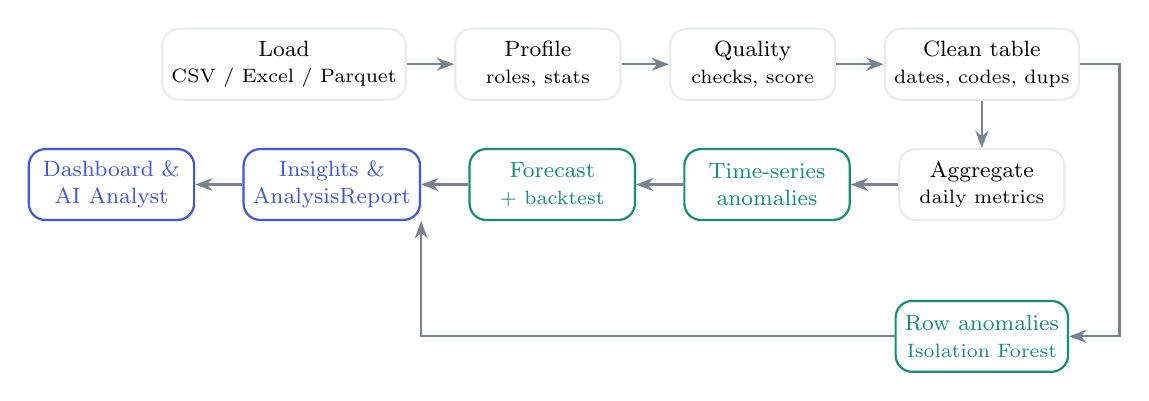
\begin{tikzpicture}[
  box/.style={draw=nsline, fill=white, rounded corners=6pt, minimum height=9mm, minimum width=21mm,
              align=center, font=\footnotesize, line width=0.8pt},
  hl/.style={box, draw=nsblue, text=nsblue},
  ml/.style={box, draw=nsteal, text=nsteal},
  arr/.style={-{Stealth[length=2.2mm]}, color=nsmuted, line width=0.8pt},
  node distance=6mm and 6mm]
  \node[box] (load) {Load\\\scriptsize CSV / Excel / Parquet};
  \node[box, right=of load] (prof) {Profile\\\scriptsize roles, stats};
  \node[box, right=of prof] (qual) {Quality\\\scriptsize checks, score};
  \node[box, right=of qual] (clean) {Clean table\\\scriptsize dates, codes, dups};
  \node[box, below=of clean] (agg) {Aggregate\\\scriptsize daily metrics};
  \node[ml, left=of agg] (ts) {Time-series\\anomalies};
  \node[ml, left=of ts] (fc) {Forecast\\\scriptsize + backtest};
  \node[ml, below=of agg, yshift=-4mm] (row) {Row anomalies\\\scriptsize Isolation Forest};
  \node[hl, left=of fc] (ins) {Insights \&\\AnalysisReport};
  \node[hl, left=of ins] (ui) {Dashboard \&\\AI Analyst};
  \draw[arr] (load) -- (prof); \draw[arr] (prof) -- (qual); \draw[arr] (qual) -- (clean);
  \draw[arr] (clean) -- (agg); \draw[arr] (agg) -- (ts); \draw[arr] (ts) -- (fc); \draw[arr] (fc) -- (ins);
  \draw[arr] (clean.east) -- ++(5mm,0) |- (row.east);
  \draw[arr] (row.west) -| (ins.south east);
  \draw[arr] (ins) -- (ui);
\end{tikzpicture}
\caption{Analysis pipeline. Blue: user-facing outputs; green: machine-learning stages.}
\label{fig:arch}
\end{figure}

\paragraph{Transactional vs.\ time-series input.} Superstore is \emph{transactional}: many rows share the same
date. Feeding it directly to a time-series model would silently drop rows. The pipeline therefore classifies a
table as transactional when the number of distinct timestamps is below $0.9\times$ the number of rows, and in that
case aggregates it per day (sum of each measure, plus row and distinct-ID counts). Superstore becomes a gap-free
daily series of \textbf{1{,}458 days} with 8 metrics, while row-level anomaly detection still runs on the full
cleaned table.

\subsection{Shared contracts}\label{sec:contracts}
All interfaces between modules are \emph{pydantic} models in \code{analyst/contracts.py}, validated on creation
(for example, a forecast must contain exactly \code{horizon} rows, an anomaly frame must have a boolean
\code{is\_anomaly} column). The main ones are:

\begin{center}
\small
\begin{tabularx}{\linewidth}{@{}lX@{}}
\toprule
Contract & Content \\
\midrule
\code{DatasetProfile} & per-column role (identifier, datetime, numeric, categorical, \dots), statistics, quality report \\
\code{QualityReport} & list of issues (check, severity, affected rows) and a 0--100 score \\
\code{AggregateResult} & the daily time series built from a transactional table \\
\code{AnomalyResult} / \code{RowAnomalyResult} & score and anomaly flag per period / per row, with a reason \\
\code{ForecastResult} & forecast with 95\% interval, backtest and baseline metrics \\
\code{AnalysisReport} & everything above plus insights and non-fatal warnings \\
\code{AnalystAnswer} & answer to a user question: intent, summary, evidence, supporting table \\
\bottomrule
\end{tabularx}
\end{center}

\subsection{Team organisation}
The project was developed with a \emph{coordinator} and three parallel agents, each working in its own Git
worktree and owning a disjoint set of files, so that no two agents edited the same file. The coordinator defined
the contracts first, reviewed each branch, and merged them one at a time, re-running the full test suite after
each merge.

\begin{center}
\small
\begin{tabularx}{\linewidth}{@{}llX@{}}
\toprule
Role & Owns & Responsibility \\
\midrule
Coordinator & \code{contracts.py}, \code{agent/}, tests & interfaces, pipeline orchestration, integration \\
Data engineering & \code{data/} & loading, profiling, quality checks, cleaning, aggregation \\
Machine learning & \code{ml/} & anomaly detection, forecasting, evaluation, benchmark \\
Dashboard & \code{dashboard/} & Streamlit user interface and charts \\
\bottomrule
\end{tabularx}
\end{center}

%-----------------------------------------------------------------------------
\section{Data engineering}

\subsection{Profiling and column roles}
Storage types are not enough to analyse a table: \code{Row ID} and \code{Postal Code} are integers but must
not be summed. The profiler assigns each column a \emph{semantic role}. A column whose values are all
distinct is an identifier; a column that parses as dates is a datetime; a numeric column with few distinct values
is categorical; and so on. Only \code{numeric} columns become analysis targets, so identifiers are never treated as
measures. For each column the profiler stores missing values, distinct values, top values, and for numeric columns
quantiles and the number of IQR outliers.

\subsection{Quality checks and score}
The quality module runs checks such as missing values, duplicate and near-duplicate rows, constant columns,
numbers stored as text, inconsistent category spellings, outliers and \emph{lost leading zeros} (for example, US
ZIP codes such as \code{01852} read as the number \code{1852}). Each issue has a severity and the score is
\[
  \text{score} = \max\!\Bigl(0,\; 100 - 10\,n_{\text{warning}} - 30\,n_{\text{error}}\Bigr),
\]
informational issues costing nothing. Superstore scores \textbf{80/100}: two warnings, namely postal codes that lost
their leading zero and one near-duplicate order line.

\subsection{Cleaning}
Cleaning is reversible and logged: every step is recorded with a description so it can be shown to the user.
For Superstore the steps are: parse the two date columns, zero-pad postal codes, strip whitespace, drop the
near-duplicate row (9{,}994 $\to$ 9{,}993 rows), aggregate per day, and interpolate the few days without orders.

\subsection{Frequency and seasonality inference}
The sampling frequency is inferred from the timestamps, and the season length follows from it: 7 for daily data
(weekly cycle), 52 for weekly, 12 for monthly, 4 for quarterly, and the number of periods per day for sub-daily
data (48 for half-hourly taxi data).

%-----------------------------------------------------------------------------
\section{Machine learning}

\subsection{Time-series anomaly detection}
Each detector computes a residual $r_t$ (what the model cannot explain) and converts it into a robust z-score
using the median absolute deviation (MAD), which, unlike the standard deviation, is not inflated by the
anomalies themselves:
\[
  z_t = \frac{\lvert r_t - \operatorname{median}(r) \rvert}{1.4826\cdot \operatorname{median}\bigl(\lvert r - \operatorname{median}(r)\rvert\bigr)},
  \qquad \text{anomaly} \iff z_t > \tau .
\]
The factor $1.4826$ makes the MAD consistent with the standard deviation for Gaussian data. Three residual
models were implemented and compared:
\begin{itemize}
  \item \textbf{Seasonal difference} (baseline): $r_t = y_t - y_{t-m}$, where $m$ is the season length.
  \item \textbf{STL}: robust Seasonal--Trend decomposition using LOESS, $y_t = T_t + S_t + r_t$, with one season.
  \item \textbf{MSTL}: STL generalised to several seasonalities, e.g.\ daily ($m=48$) and weekly ($m=336$) for
        half-hourly data.
\end{itemize}
The default is the seasonal difference with $\tau = 3.5$. For sub-daily series with at least eight weeks of
history the pipeline switches automatically to MSTL with $\tau = 4$, the best setting on the benchmark.

\subsection{Row-level anomaly detection}
Aggregated series can hide individual suspicious orders, so the cleaned table is also scored row by row with an
\textbf{Isolation Forest} (scikit-learn, 200 trees). Features are the numeric columns plus a derived
\textbf{profit margin} $\text{Profit}/\text{Sales}$, which exposes orders that are normal in size but sold at a
loss. Each feature is centred on its median, divided by its MAD and compressed with $\operatorname{asinh}$ to tame
heavy tails. The rows with the top $1\%$ of anomaly scores are flagged, and each flagged row receives a readable
reason, for example \emph{``Sales 22{,}638 (very high), Profit $-1{,}811$ (very low)''}.

\subsection{Forecasting}
The first forecasting model is a \textbf{seasonal naive} model, which repeats the last observed season:
$\hat y_{T+h} = y_{T+h-m\lceil h/m\rceil}$. A 95\% interval is built as $\hat y \pm 1.96\,\sigma$, with $\sigma$
the standard deviation of seasonal differences. The model is validated with a hold-out backtest over the last
$H=48$ days and compared with a last-value naive baseline using MAE, RMSE and MAPE.

%-----------------------------------------------------------------------------
\section{Evaluation}

\subsection{Time-series anomalies on NYC taxi}
Table~\ref{tab:taxi} reports point-wise precision, recall and F1 against the NAB labels, and \emph{event recall}
(the share of the five labelled events in which at least one point is flagged).

\begin{table}[H]
\centering\small
\begin{tabular}{@{}lccccccc@{}}
\toprule
Method & $\tau$ & Precision & Recall & F1 & Event recall & \% flagged \\
\midrule
Seasonal difference (baseline) & 3.5 & 0.198 & 0.205 & 0.201 & 1.00 & 10.4 \\
STL, daily season              & 4.0 & 0.151 & 0.281 & 0.196 & 1.00 & 18.7 \\
STL, weekly season ($m=336$)   & 4.0 & 0.324 & 0.507 & 0.395 & 1.00 & 15.7 \\
\textbf{MSTL, daily + weekly}  & \textbf{4.0} & \textbf{0.388} & \textbf{0.480} & \textbf{0.429} & \textbf{1.00} & \textbf{12.4} \\
MSTL + 1-day score smoothing   & 4.0 & 0.560 & 0.588 & 0.574 & 1.00 & 10.5 \\
\bottomrule
\end{tabular}
\caption{Anomaly detection on NYC taxi (10{,}320 half-hourly points, 5 labelled events).}
\label{tab:taxi}
\end{table}

\noindent
Modelling both seasonalities more than doubles the F1 score of the baseline (0.429 vs.\ 0.201) while flagging
fewer points. Smoothing the score over one day improves the point metrics further because the NAB labels are
windows rather than single points; it was kept as an option rather than a default.

\subsection{Row anomalies on Superstore with injected anomalies}
Fifty synthetic anomalous orders of four kinds (huge sales, large discount with a loss, negative margin, bulk
quantity) were injected into Superstore, and each method flags $1\%$ of the rows.

\begin{table}[H]
\centering\small
\begin{tabular}{@{}lccc@{}}
\toprule
Method (contamination $1\%$) & Precision & Recall & F1 \\
\midrule
Max robust z-score per feature           & 0.307 & 0.620 & 0.411 \\
Isolation Forest, no asinh compression   & 0.178 & 0.360 & 0.238 \\
Isolation Forest, asinh-scaled features  & 0.465 & 0.940 & 0.623 \\
\textbf{Isolation Forest, scaled + profit margin} & \textbf{0.495} & \textbf{1.000} & \textbf{0.662} \\
\bottomrule
\end{tabular}
\caption{Row-level anomaly detection on Superstore with 50 injected anomalous orders.}
\end{table}

\noindent
Feature scaling and the domain-specific margin ratio matter more than the choice of algorithm: the margin feature
alone raises recall on negative-margin orders from 0.75 to 1.00. Precision is bounded by the budget: flagging
$1\%$ of about 10{,}000 rows yields about 100 rows for 50 true anomalies, so the maximum achievable precision is
about 0.5.

\subsection{Results on Superstore}
On the real data the pipeline flags \textbf{100 of 9{,}993 order lines} (1\%) and 123 unusual days of sales (8.4\%).
The latter figure is high for business data and is discussed in Section~\ref{sec:future}. For the 48-day forecast
backtest, the seasonal naive model beats the naive baseline on sales (MAE 1{,}916 vs.\ 2{,}220, $-14\%$) and on quantity
(MAE 24.6 vs.\ 44.2), but not on profit or discount, which have no clear weekly pattern. The dashboard reports this
comparison honestly with each forecast.

%-----------------------------------------------------------------------------
\section{User interface: the Northstar dashboard}

The interface is a Streamlit application with a custom design system (Northstar): a light canvas, white cards,
a blue/teal/amber palette, and a left navigation rail with four pages. It loads the Superstore sample on start
and can analyse any uploaded CSV, Excel or Parquet file.

\begin{figure}[H]
\centering
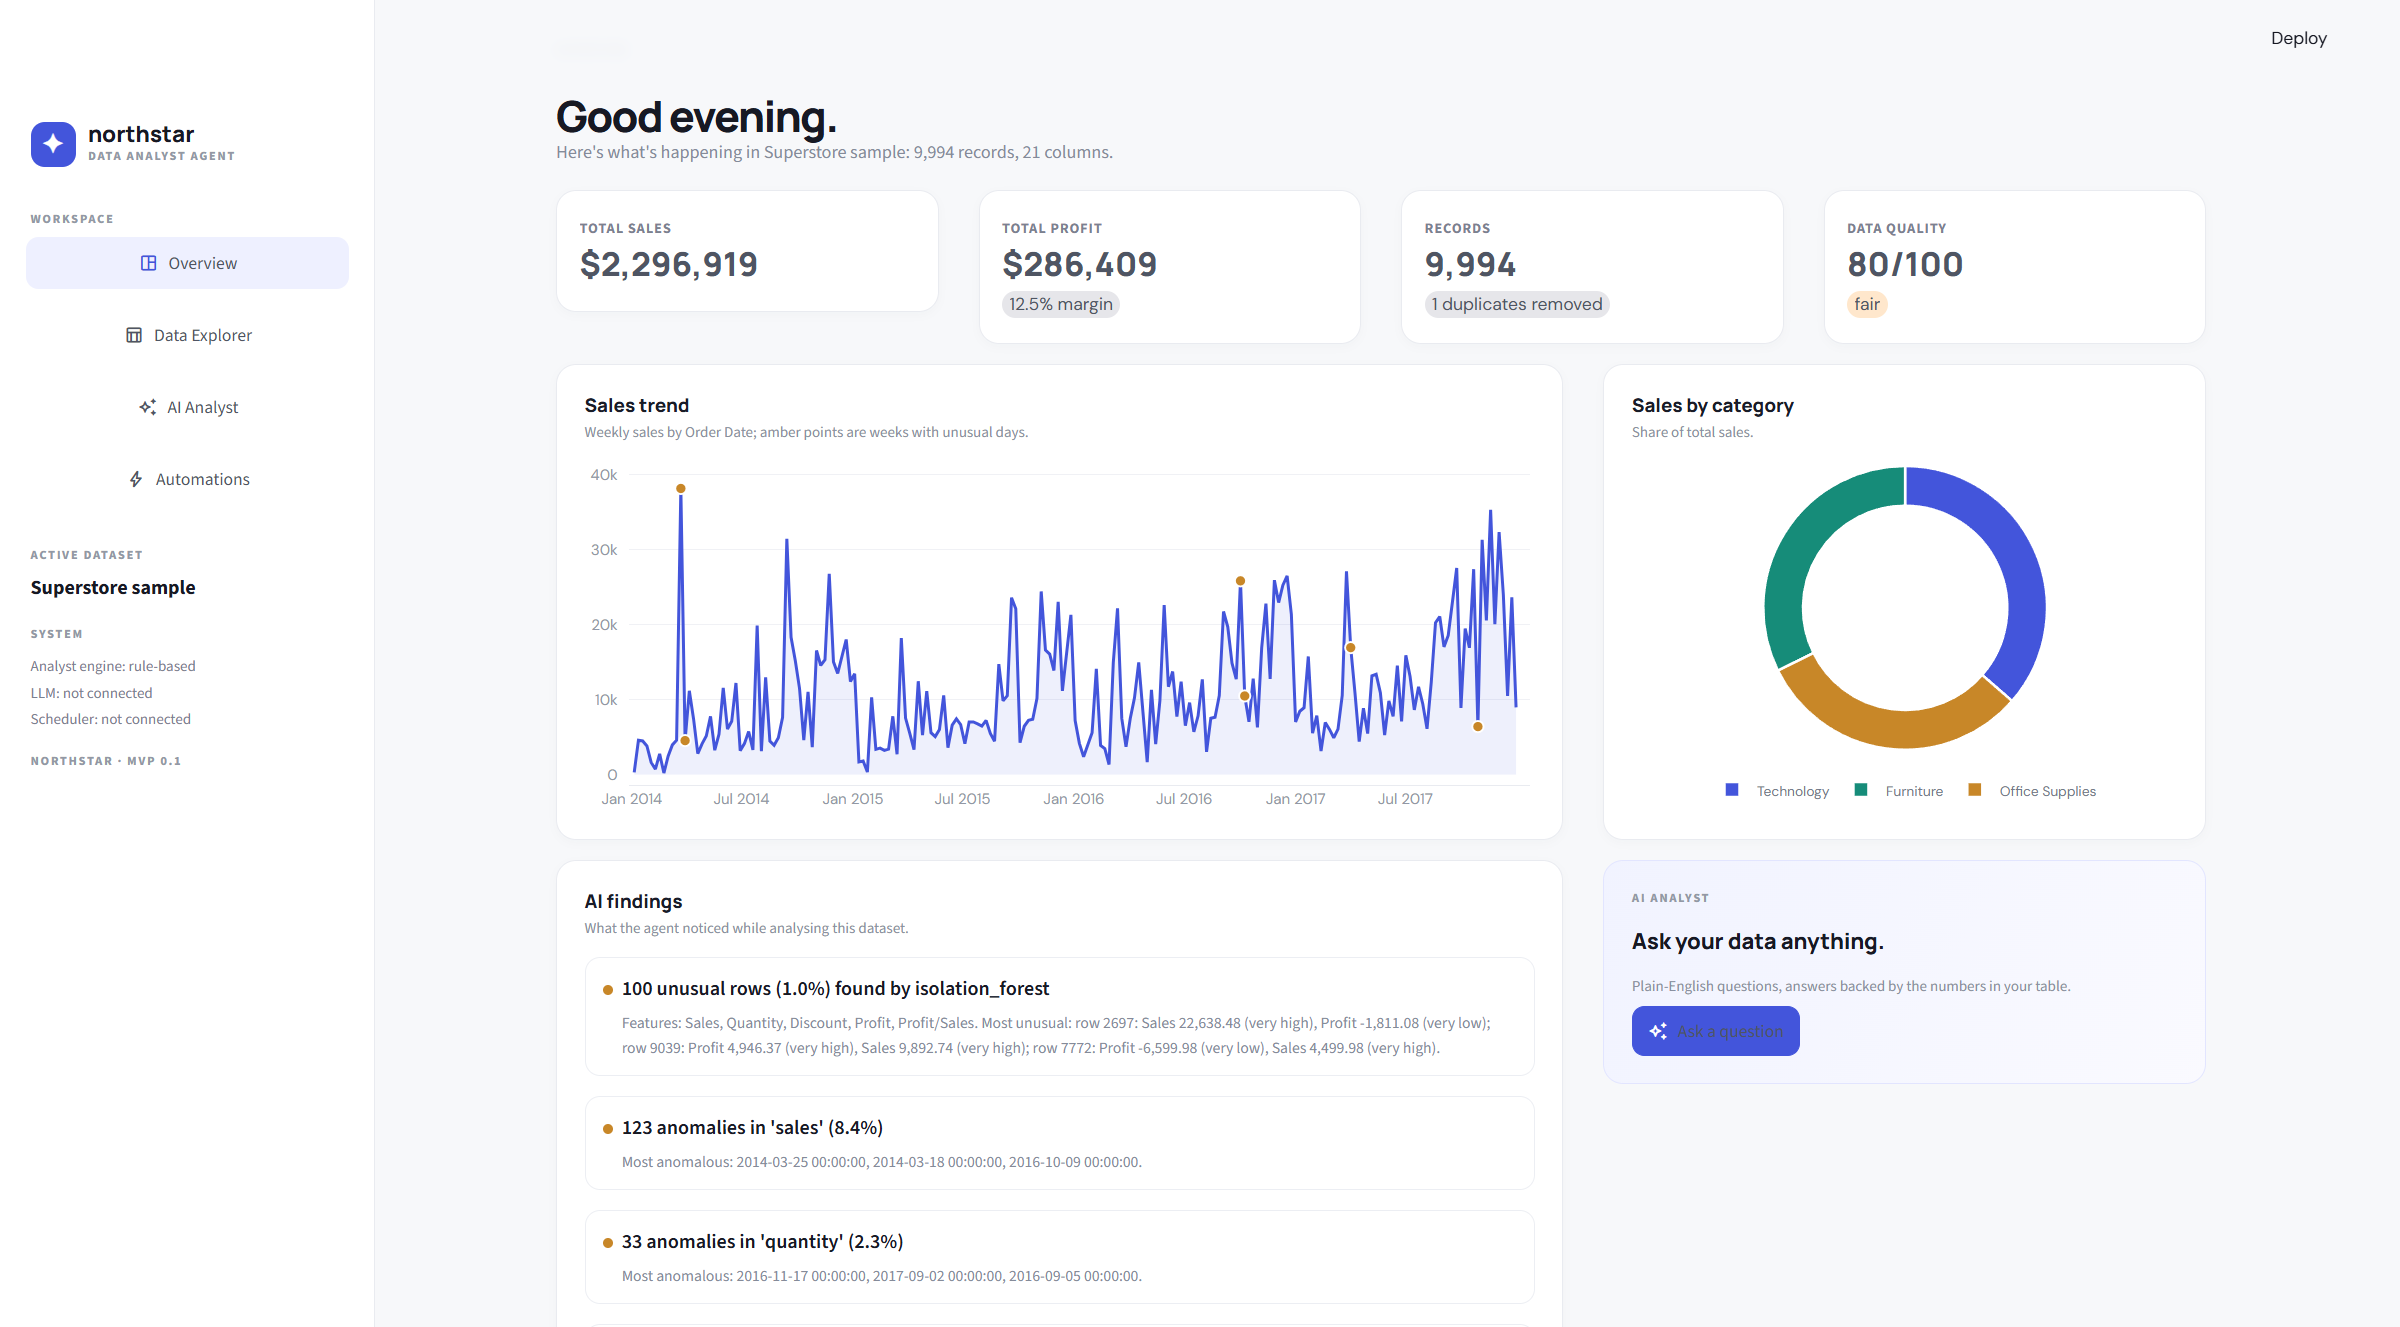
\includegraphics[width=\linewidth]{overview.png}
\caption{Overview: headline indicators, weekly sales trend (amber points mark weeks containing anomalous days),
sales by category, and the findings generated by the agent.}
\end{figure}

\begin{figure}[H]
\centering
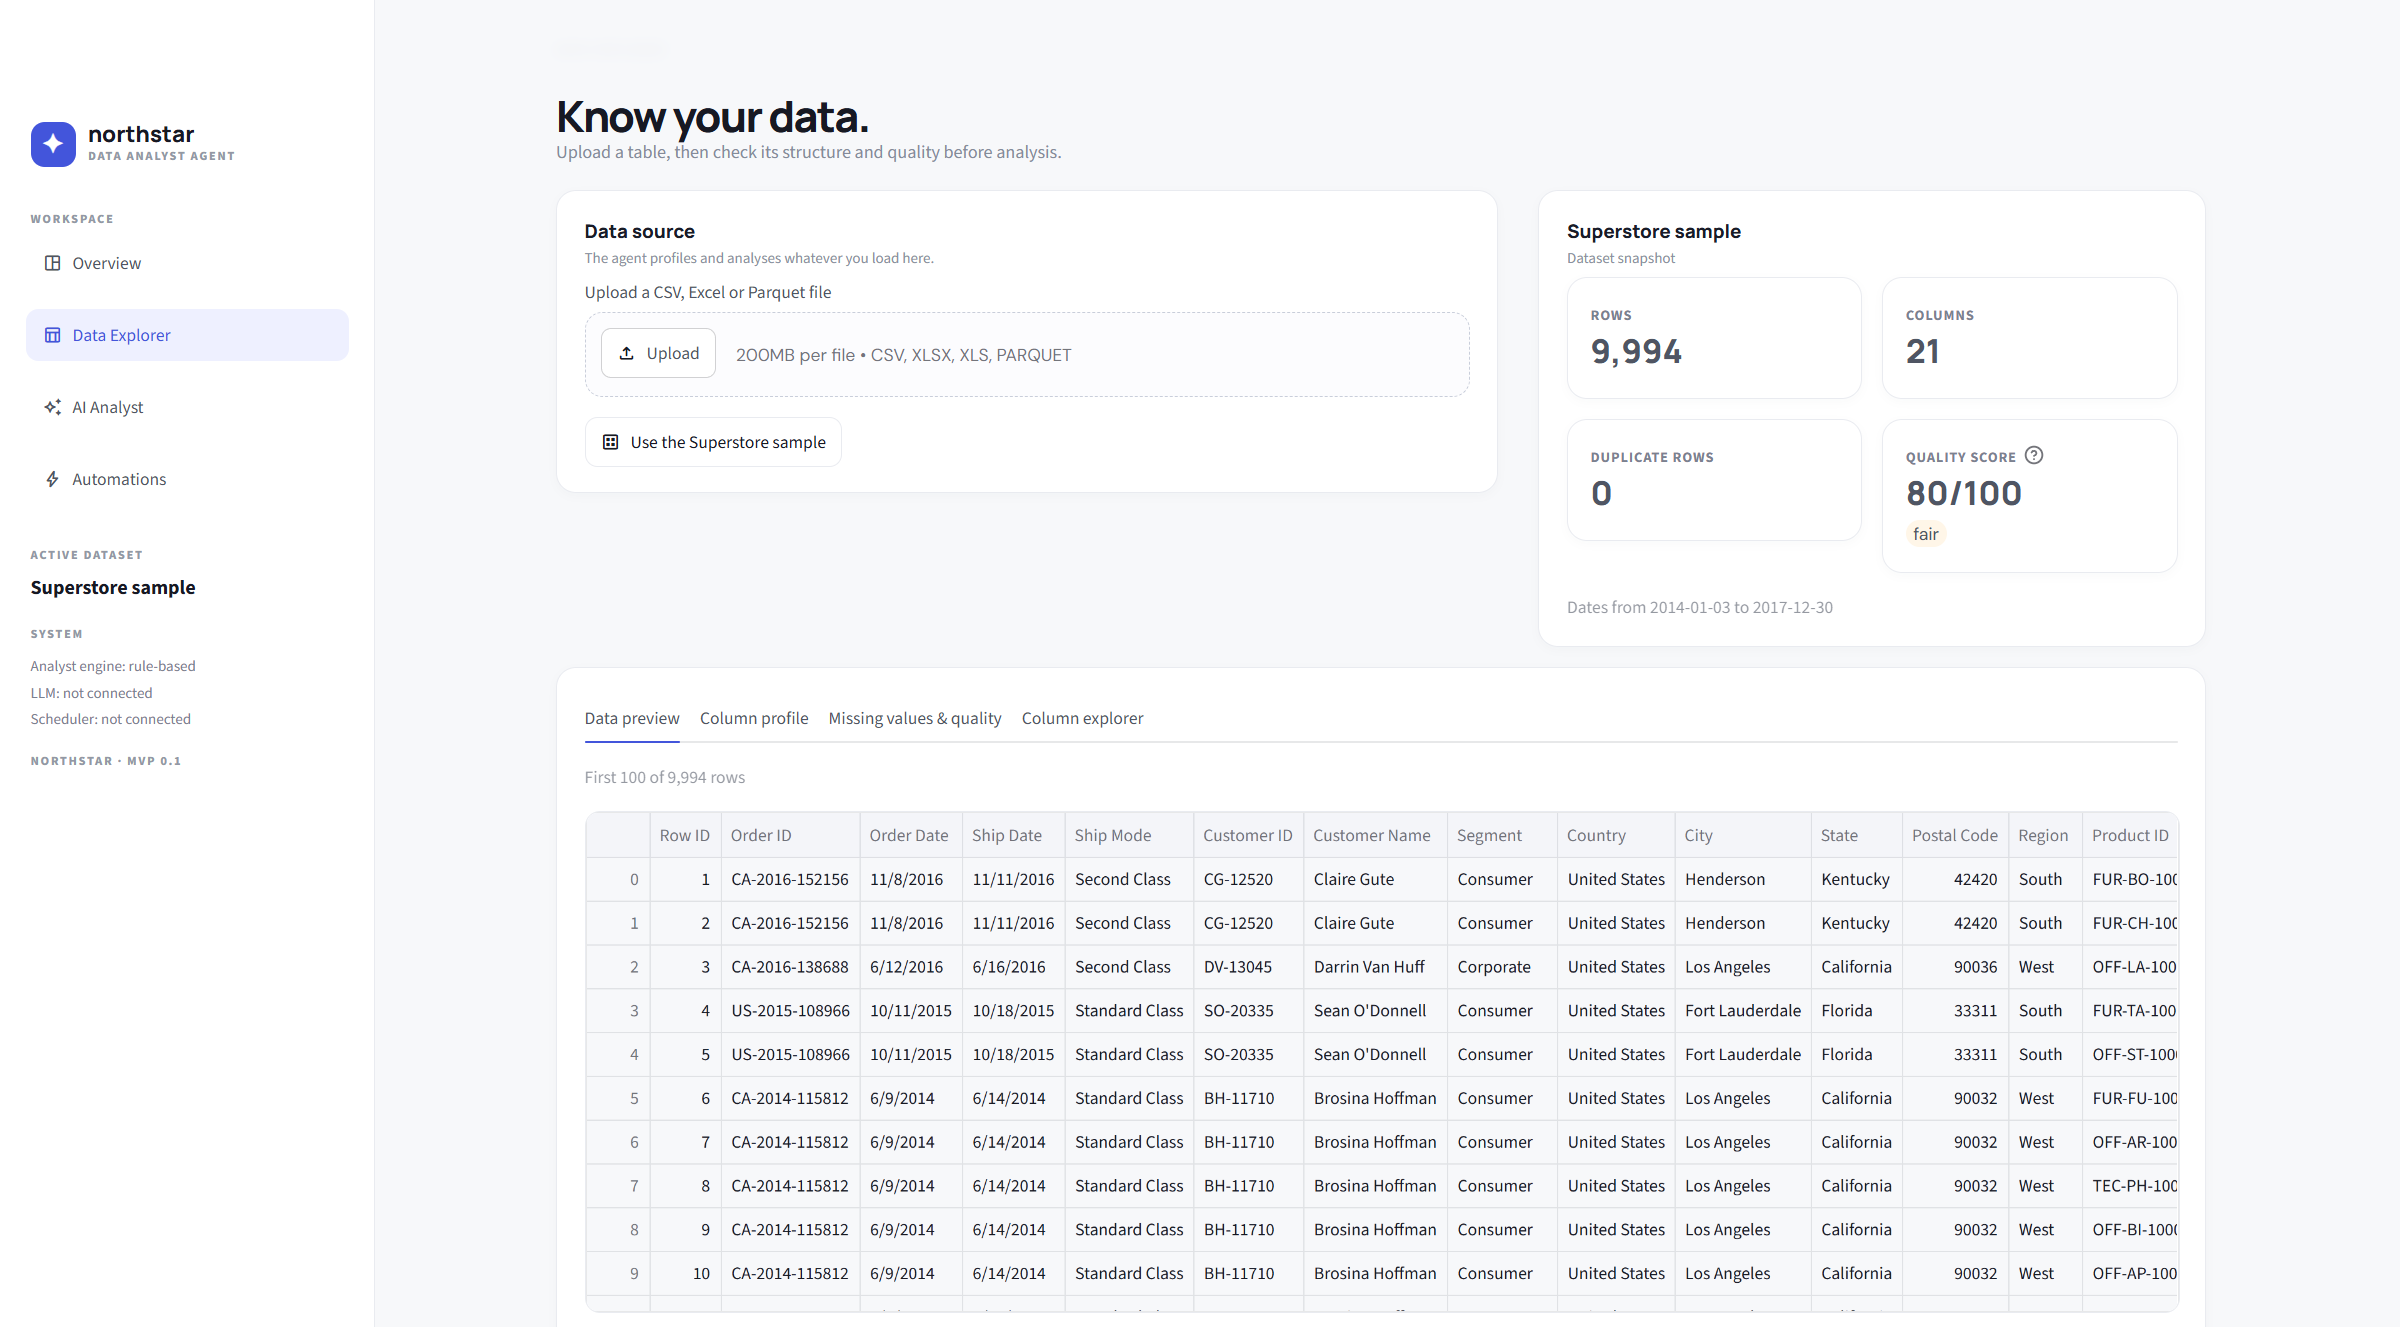
\includegraphics[width=\linewidth]{explorer.png}
\caption{Data Explorer: upload, dataset snapshot (rows, columns, duplicates, quality score) and tabs for the
data preview, column profile, quality issues and a per-column explorer.}
\end{figure}

\begin{figure}[H]
\centering
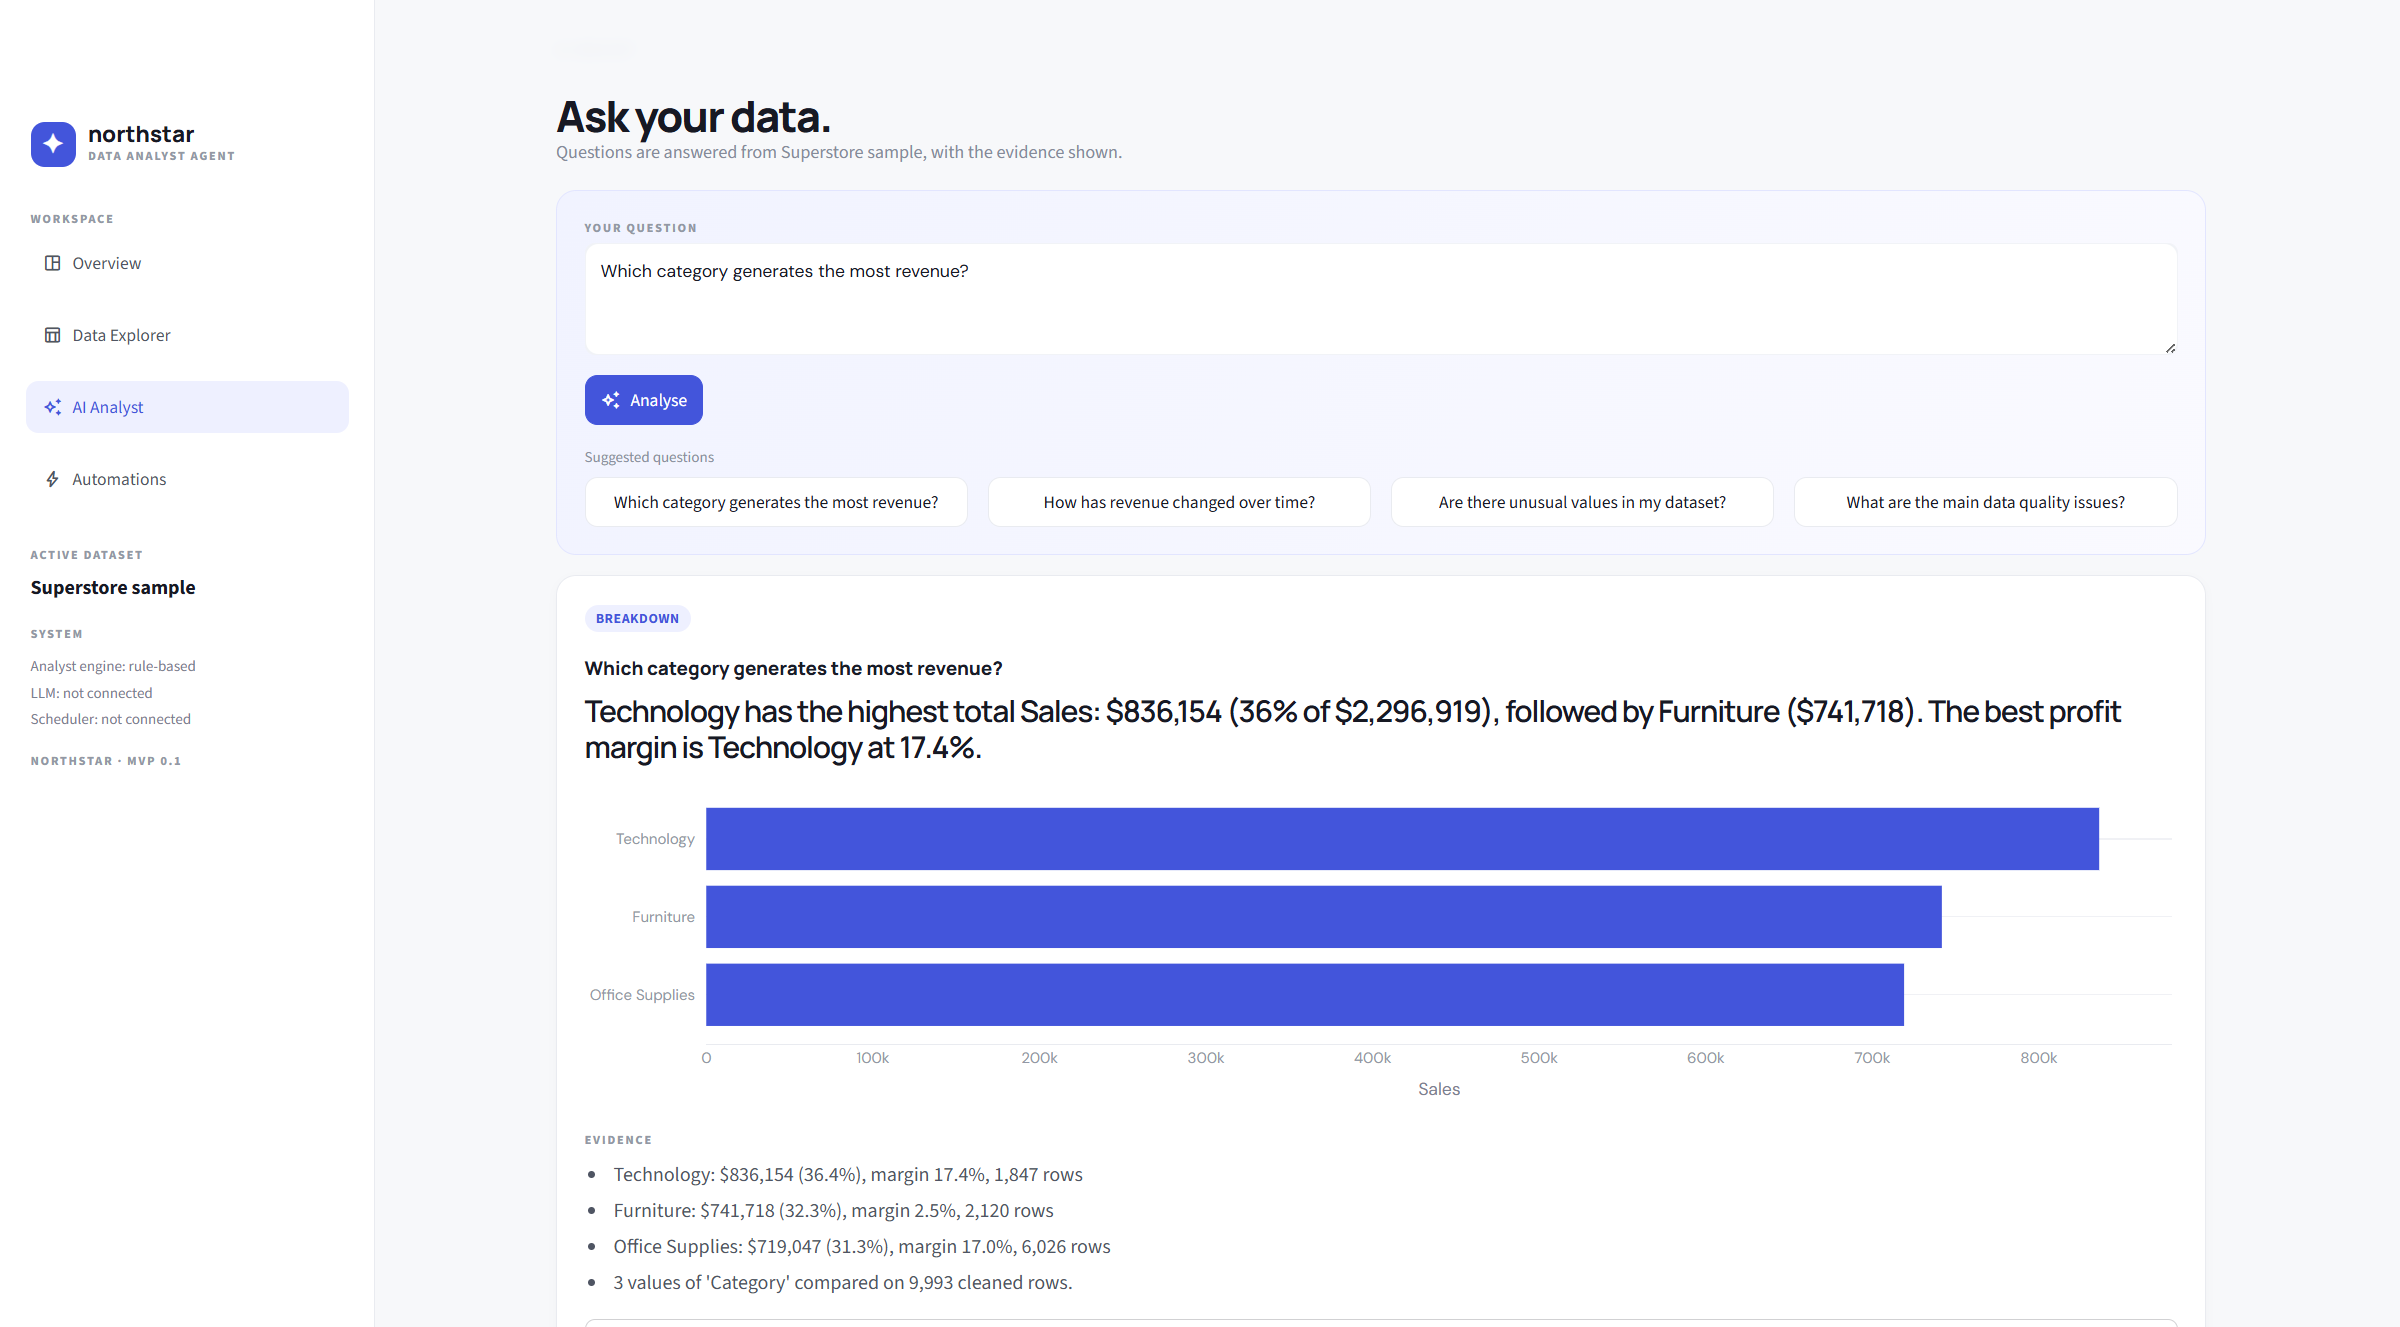
\includegraphics[width=\linewidth]{ai_analyst.png}
\caption{AI Analyst: the question ``Which category generates the most revenue?'' is answered with a summary, a
chart, the supporting evidence and the underlying table.}
\end{figure}

\subsection{AI Analyst}
Questions are routed to one of six intents: \emph{breakdown}, \emph{trend}, \emph{anomalies}, \emph{quality},
\emph{forecast} and \emph{overview}. The analyst then finds the relevant measure (``revenue'' maps to
\code{Sales}) and dimension (e.g.\ \code{Category}) from the profile, computes the answer with pandas, and
returns an \code{AnalystAnswer}. Example answers on Superstore:
\begin{itemize}
  \item \emph{Which category generates the most revenue?} Technology, \$836{,}154 (36\% of sales), with the
        best margin (17.4\%); Furniture follows with \$741{,}718 but only a 2.5\% margin.
  \item \emph{How has revenue changed over time?} Sales grew by 20.4\% from 2016 to 2017; the best month was
        November 2017 (\$118{,}448).
  \item \emph{Are there unusual values in my dataset?} 100 of 9{,}993 rows flagged, each with its reason.
  \item \emph{What are the main data quality issues?} Score 80/100, with the issues and the cleaning steps applied.
\end{itemize}
The current engine is deterministic and rule-based. It was designed behind the same contract as the planned LLM
agent, so the language model can be added without changing the interface; the engine in use is always displayed
under each answer.

\subsection{Automations}
The fourth page lets the user save recurring checks (full report, anomaly check, quality check or revenue trend)
with a cadence and a destination, and run them on demand with \emph{Run now}. Scheduled execution is the next
step (APScheduler); the page states clearly that the scheduler is not yet connected.

%-----------------------------------------------------------------------------
\section{Software engineering and testing}

\begin{itemize}
  \item \textbf{Stack}: Python, pandas 3, NumPy, scikit-learn, statsmodels (STL/MSTL), pydantic, Streamlit,
        Plotly, Git.
  \item \textbf{Tests}: 176 automated tests (pytest) cover the contracts, each data and ML module, the full
        pipeline on Superstore and NYC taxi, the AI analyst answers, and every dashboard page through Streamlit's
        \code{AppTest} (navigation, KPIs, a question/answer round trip, creating and running an automation).
        The suite also runs with pandas deprecation warnings turned into errors.
  \item \textbf{Integration discipline}: each agent's branch was reviewed and merged only when the full suite
        passed, so the application kept working after every merge.
\end{itemize}

\paragraph{Problems found during integration.} Several issues were found by testing on real data rather than toy
examples:
\begin{itemize}
  \item The first pipeline treated Superstore as a time series and dropped 88\% of the rows (9{,}994 $\to$ 1{,}237
        dates); transactional detection and aggregation fixed this.
  \item Identifier columns (\code{Row ID}, \code{Postal Code}) were initially picked as analysis targets;
        targets are now chosen from semantic roles.
  \item With pandas 3 the daily frequency is no longer a fixed-length offset, which silently disabled season
        detection and made the seasonal forecast identical to the naive one; season inference was rewritten.
  \item Making MSTL the global default over-flagged Superstore (14--18\% of days), so it is applied only where the
        benchmark supports it (long sub-daily series).
\end{itemize}

%-----------------------------------------------------------------------------
\section{Limitations and future work}\label{sec:future}

\begin{itemize}
  \item \textbf{LLM reasoning layer}: replace the rule-based analyst with a LangGraph agent using Gemini that
        calls the existing analysis functions as tools, keeping answers grounded in computed numbers.
  \item \textbf{Anomalies on business series}: about 8\% of days are flagged on Superstore's daily sales,
        because daily retail sales are very irregular. Weekly aggregation or a higher threshold for transactional
        data should be evaluated.
  \item \textbf{Forecasting}: add stronger models (ETS, gradient boosting with calendar features) and replace
        MAPE, which is unreliable on days with near-zero sales, by a scaled error such as MASE.
  \item \textbf{Product features}: SQLite analysis history, APScheduler for scheduled automations, alerts by
        e-mail or Slack, and SQL database sources.
\end{itemize}

%-----------------------------------------------------------------------------
\section{Demonstration script}

\begin{enumerate}
  \item Start the app:
\begin{lstlisting}[language=bash]
.\.venv\Scripts\streamlit run src/analyst/dashboard/app.py
\end{lstlisting}
  \item \textbf{Overview}: point out the indicators (\$2.30M sales, 12.5\% margin, quality 80/100), the amber
        anomaly markers on the trend and the agent's findings.
  \item \textbf{Data Explorer}: open the quality tab (lost leading zeros in postal codes, near-duplicate row) and the
        column explorer on \code{Profit} (distribution and outliers).
  \item \textbf{AI Analyst}: click the four suggested questions; for the anomaly question, show the reasons
        attached to flagged rows.
  \item \textbf{Automations}: create a weekly anomaly check and press \emph{Run now}.
  \item Close with the benchmark tables: MSTL 0.429 vs.\ 0.201 F1, and Isolation Forest recall 1.00 with the
        margin feature.
\end{enumerate}

%-----------------------------------------------------------------------------
\section{Conclusion}
The project delivers a working autonomous analyst for tabular business data. A file goes in; out come a profile,
a quality score, cleaned data, anomalies at both the day and the order level, a forecast, and plain-English
answers backed by evidence, all in a polished web interface. The main lesson is that \emph{data understanding
drives model quality}. Detecting transactional tables, choosing targets by semantic role, and adding a single
domain feature (profit margin) had a larger effect on the results than switching algorithms, and every one of
these problems was caught by testing on the real dataset.

\end{document}
